\documentclass[10pt,handout,hyperref={unicode}]{beamer}

%-------------------------------------------------------
% Beamer Theme location override
%-------------------------------------------------------

\makeatletter
  \def\beamer@calltheme#1#2#3{%
    \def\beamer@themelist{#2}
    \@for\beamer@themename:=\beamer@themelist\do
    {\usepackage[{#1}]{\beamer@themelocation/#3\beamer@themename}}}

  \def\usefolder#1{
    \def\beamer@themelocation{#1}
  }
  \def\beamer@themelocation{}

%-------------------------------------------------------
% INCLUDE PACKAGES
%-------------------------------------------------------

\usepackage{minted} % Code listing
\usepackage{forest} % Tree graphs
\usepackage{fontspec} % UTf-8 input support lualatex
% \usepackage{multirow}
\usepackage{hyperref}
\usepackage{wasysym}
\usepackage[absolute,overlay]{textpos}
\usepackage{graphicx}
\usepackage{microtype} % nice text appearance
\usepackage{ragged2e}
\usepackage{pgfpages}
\usepackage[ngerman]{babel} % german text standards
\usepackage{docmute} % Import other .tex files ignoring document
\usepackage{multicol} % Automatically use multiple columns
\usepackage{fontawesome} % WebFonts including href icon

%-------------------------------------------------------
% Config Theme
%-------------------------------------------------------
\usefolder{../Templates/featherZR}
\usetheme[
    progressstyle=movingCircCnt   % fixedCircCnt, movingCircCnt (moving is deault)
  ]{Feather}

\setsansfont{HelveticaNeue}
\setmonofont{Source Code Pro for Powerline}[Scale = MatchLowercase]

%-------------------------------------------------------
% DEFFINING AND REDEFINING COMMANDS
%-------------------------------------------------------

%\setbeameroption{show notes}
%\setbeameroption{show notes on second screen=right}

%Set Path to images
\graphicspath{{Images/}}

% colored hyperlinks
\newcommand{\chref}[2]{%
\href{#1}{{\usebeamercolor[bg]{Feather}#2} {\footnotesize\faExternalLink}}%
}

%Justification
\addtobeamertemplate{theorem begin}{}{\justifying}
\addtobeamertemplate{block begin}{}{\justifying}
\addtobeamertemplate{itemize begin}{}{\justifying}
\addtobeamertemplate{item begin}{}{\justifying}
\addtobeamertemplate{frame begin}{}{\justifying}
\addtobeamertemplate{quote begin}{}{\justifying}
\addtobeamertemplate{structure begin}{}{\justifying}

%etoolbox für nested list covering
\setbeamercovered{transparent}

%description inde
\setbeamersize{description width=0.57cm}

\makeatletter
\newcommand*\fix@beamer@close{%
  \ifnum\beamer@trivlistdepth>0
  \beamer@closeitem
  \fi
}
\newcommand*\fix@beamer@open{%
  \ifnum\beamer@trivlistdepth>0
  \gdef\beamer@closeitem{}%
  \fi
}
\newcommand<>{\highlighton}[1]{%
  \alt#2{\structure{#1}}{{#1}}
}

\BeforeBeginEnvironment{enumerate}{\fix@beamer@close}
\AfterEndEnvironment{enumerate}{\fix@beamer@open}
\BeforeBeginEnvironment{itemize}{\fix@beamer@close}
\AfterEndEnvironment{itemize}{\fix@beamer@open}
\BeforeBeginEnvironment{description}{\fix@beamer@close}
\AfterEndEnvironment{description}{\fix@beamer@open}
\makeatother

% Codelistings
\definecolor{monokaibg}{HTML}{002833}
\definecolor{highlightbg}{HTML}{004550}

\setminted{
  autogobble=true,
  bgcolor=monokaibg,
  breaklines=true,
  fontsize=\footnotesize,
  highlightcolor=highlightbg,
  linenos=true,
  labelposition=bottomline,
  rulecolor=white,
  style=native,
}

\setmintedinline{
  bgcolor={},
  fontsize=\normalsize,
  style=manni
}

%-------------------------------------------------------
% INFORMATION IN THE TITLE PAGE
%-------------------------------------------------------

\title[PHPUnit Tutorial ] % [] is optional - is placed on the bottom of the sidebar on every slide
{ % is placed on the title page
      \textbf{PHPUnit Tutorial}
}

\subtitle[ -- Funktionsweise von PHPUnit]
{
%      \textbf{v. 1.0.0}
}

\author[Sebastian Knott]{Sebastian Knott}

\institute[]
{
      ZooRoyal IT\\

  %there must be an empty line above this line - otherwise some unwanted space is added between the university and the country (I do not know why;( )
}

\date{\today}

\begin{document}

\documentclass[10pt,hyperref={unicode}]{beamer}

%!TeX spellcheck = en-US,de-DE

%-------------------------------------------------------
% Beamer Theme location override
%-------------------------------------------------------

\makeatletter
  \def\beamer@calltheme#1#2#3{%
    \def\beamer@themelist{#2}
    \@for\beamer@themename:=\beamer@themelist\do%
    {\usepackage[{#1}]{\beamer@themelocation/#3\beamer@themename}}}

  \def\usefolder#1{
    \def\beamer@themelocation{#1}
  }
  \def\beamer@themelocation{}

%-------------------------------------------------------
% INCLUDE PACKAGES
%-------------------------------------------------------

\usepackage{minted} % Code listing
\usepackage{forest} % Tree graphs
\usepackage{fontspec} % UTF-8 input support lualatex
% \usepackage{multirow}
\usepackage{hyperref}
\usepackage{wasysym}
\usepackage[absolute,overlay]{textpos}
\usepackage{graphicx}
\usepackage{microtype} % nice text appearance
\usepackage{ragged2e}
\usepackage{pgfpages}
\usepackage[ngerman]{babel} % German text standards
\usepackage{docmute} % Import other .tex files ignoring document
\usepackage{multicol} % Automatically use multiple columns
\usepackage{fontawesome} % Web Fonts including href icon
\usepackage[normalem]{ulem} % Strike through text

%-------------------------------------------------------
% Config Theme
%-------------------------------------------------------
\usefolder{../Templates/featherZR}
\usetheme[
    progressstyle=movingCircCnt   % fixedCircCnt, movingCircCnt (moving is deault)
  ]{Feather}

\setsansfont{HelveticaNeue}
\setmonofont{Source Code Pro for Powerline}[Scale = MatchLowercase]

%-------------------------------------------------------
% DEFFINING AND REDEFINING COMMANDS
%-------------------------------------------------------

% Set notes frames
\setbeameroption{show notes}
\setbeameroption{show notes on second screen=right}

%Set Path to images
\graphicspath{{Images/}}

% colored hyperlinks
\newcommand{\chref}[2]{%
\href{#1}{{\usebeamercolor[bg]{Feather}#2} {\footnotesize\faExternalLink}}%
}

%Justification
\addtobeamertemplate{theorem begin}{}{\justifying}
\addtobeamertemplate{block begin}{}{\justifying}
\addtobeamertemplate{itemize begin}{}{\justifying}
\addtobeamertemplate{item begin}{}{\justifying}
\addtobeamertemplate{frame begin}{}{\justifying}
\addtobeamertemplate{quote begin}{}{\justifying}
\addtobeamertemplate{structure begin}{}{\justifying}

%etoolbox für nested list covering
\setbeamercovered{transparent}

%description inde
\setbeamersize{description width=0.57cm}

\makeatletter
\newcommand*\fix@beamer@close{%
  \ifnum\beamer@trivlistdepth>0
  \beamer@closeitem%
  \fi
}
\newcommand*\fix@beamer@open{%
  \ifnum\beamer@trivlistdepth>0
  \gdef\beamer@closeitem{}%
  \fi
}
\newcommand<>{\highlighton}[1]{%
  \alt#2{\structure{#1}}{{#1}}
}

\BeforeBeginEnvironment{enumerate}{\fix@beamer@close}
\AfterEndEnvironment{enumerate}{\fix@beamer@open}
\BeforeBeginEnvironment{itemize}{\fix@beamer@close}
\AfterEndEnvironment{itemize}{\fix@beamer@open}
\BeforeBeginEnvironment{description}{\fix@beamer@close}
\AfterEndEnvironment{description}{\fix@beamer@open}
\makeatother

% Codelistings
\definecolor{monokaibg}{HTML}{002833}
\definecolor{highlightbg}{HTML}{004550}

\setminted{
  autogobble=true,
  bgcolor=monokaibg,
  breaklines=true,
  fontsize=\footnotesize,
  highlightcolor=highlightbg,
  linenos=true,
  labelposition=bottomline,
  rulecolor=white,
  style=native,
  xleftmargin=\parindent{}
}

\setmintedinline{
  bgcolor={},
  fontsize=\normalsize,
  style=manni
}

% multicols column separator
\setlength{\columnsep}{2em}

%-------------------------------------------------------
% INFORMATION IN THE TITLE PAGE
%-------------------------------------------------------

\title[Xdebug ] % [] is optional - is placed on the bottom of the sidebar on every slide
{ % is placed on the title page
      \textbf{Xdebug}
}

\subtitle[ -- Funktionsweise von PHPUnit]
{
%      \textbf{v. 1.0.0}
}

\author[Sebastian Knott]{Sebastian Knott}

\institute[]
{
      ZooRoyal IT\\

  %there must be an empty line above this line - otherwise some unwanted space is added between the university and the country (I do not know why;( )
}

\date{\today}

%-------------------------------------------------------
% THE TITLE OF THE PRESENTATION
%-------------------------------------------------------

\begin{document}

{\1
\begin{frame}[plain,noframenumbering] % the plain option removes the header from the title page, noframenumbering removes the numbering of this frame only
  \titlepage{} % call the title page information from above
\end{frame}}

% \AtBeginSection[]
% {
%   \frame<handout:0>
%   {
%     \frametitle{Überblick}
%     \tableofcontents[currentsection,hideothersubsections,sectionstyle=show/shaded,subsectionstyle=show/shaded]
%   }
% }

\AtBeginSubsection[]
{
  \frame<handout:0>
  {
    \frametitle{Überblick}
    \begin{columns}
      \begin{column}{0.5\textwidth}
        \begin{figure}
          \begin{center}
            
\includegraphics[width=0.9\textwidth]{logo-php}
          \end{center}
        \end{figure}
      \end{column}
      \begin{column}{0.5\textwidth}
        % \begin{multicols}{2}
          \tableofcontents[currentsection,sectionstyle=show/shaded,subsectionstyle=show/shaded,subsubsectionstyle=shaded/shaded/hide]
        % \end{multicols}
      \end{column}
    \end{columns}
  }
}

\AtBeginSubsubsection[]
{
  \frame<handout:0>
  {
    \frametitle{Überblick}
    \begin{columns}[onlytextwidth]
      \begin{column}{0.5\textwidth}
        \begin{figure}
          \begin{center}
            
\includegraphics[width=0.9\textwidth]{logo-php}
          \end{center}
        \end{figure}
      \end{column}
      \begin{column}{0.5\textwidth}
        % \begin{multicols}{2}
          \tableofcontents[currentsection,sectionstyle=show/shaded,subsectionstyle=show/shaded,subsubsectionstyle=show/shaded/hide]
        % \end{multicols}
      \end{column}
    \end{columns}
  }
}

%-------------------------------------------------------
% THE BODY OF THE PRESENTATION
%-------------------------------------------------------

\begin{frame}
  \frametitle{Überblick}
  \begin{columns}
    \begin{column}{0.5\textwidth}
      \begin{figure}
        \begin{center}
          
\includegraphics[width=0.9\textwidth]{logo-php}
        \end{center}
      \end{figure}
    \end{column}
    \begin{column}{0.5\textwidth}
      % \begin{multicols}{2}
        \tableofcontents[currentsection,sectionstyle=show,subsectionstyle=show/shaded,subsubsectionstyle=hide]
      % \end{multicols}
    \end{column}
  \end{columns}
\end{frame}

\section{Bevor es los geht}
\subsection{Was ist Xdebug}


\begin{frame}
    \frametitle{\secname}
    \framesubtitle{\subsecname}

    \begin{block}{}
      \begin{quotation}
        Xdebug is an extension for PHP to assist with debugging and development.
        \note[item] {Erweiterung unterstützt bei der Entwicklung}
        It contains a single step debugger to use with IDEs;
        \note[item] {Debugger}
        it upgrades PHP's \mintinline{php}|var_dump()| function; it adds stack traces for Notices, Warnings, Errors and Exceptions;
        \note[item] {Erweitert die Ausgabe von Fehlern}
        it features functionality for recording every function call and variable assignment to disk; it contains a profiler;
        \note[item] {Zeichnet auf wunsch den Ablauf einer Application auf}
        and it provides code coverage functionality for use with PHPUnit.
        \note[item] {Ermö glicht PHPUnit Code Coverage analyse}
        \end{quotation}
        \flushright{{\em -- \chref{https://xdebug.org/}{xdebug.org}}}
    \end{block}
\end{frame}


\begin{frame}
    \frametitle{\subsecname}
    \framesubtitle{Debugging}

    \begin{figure}
      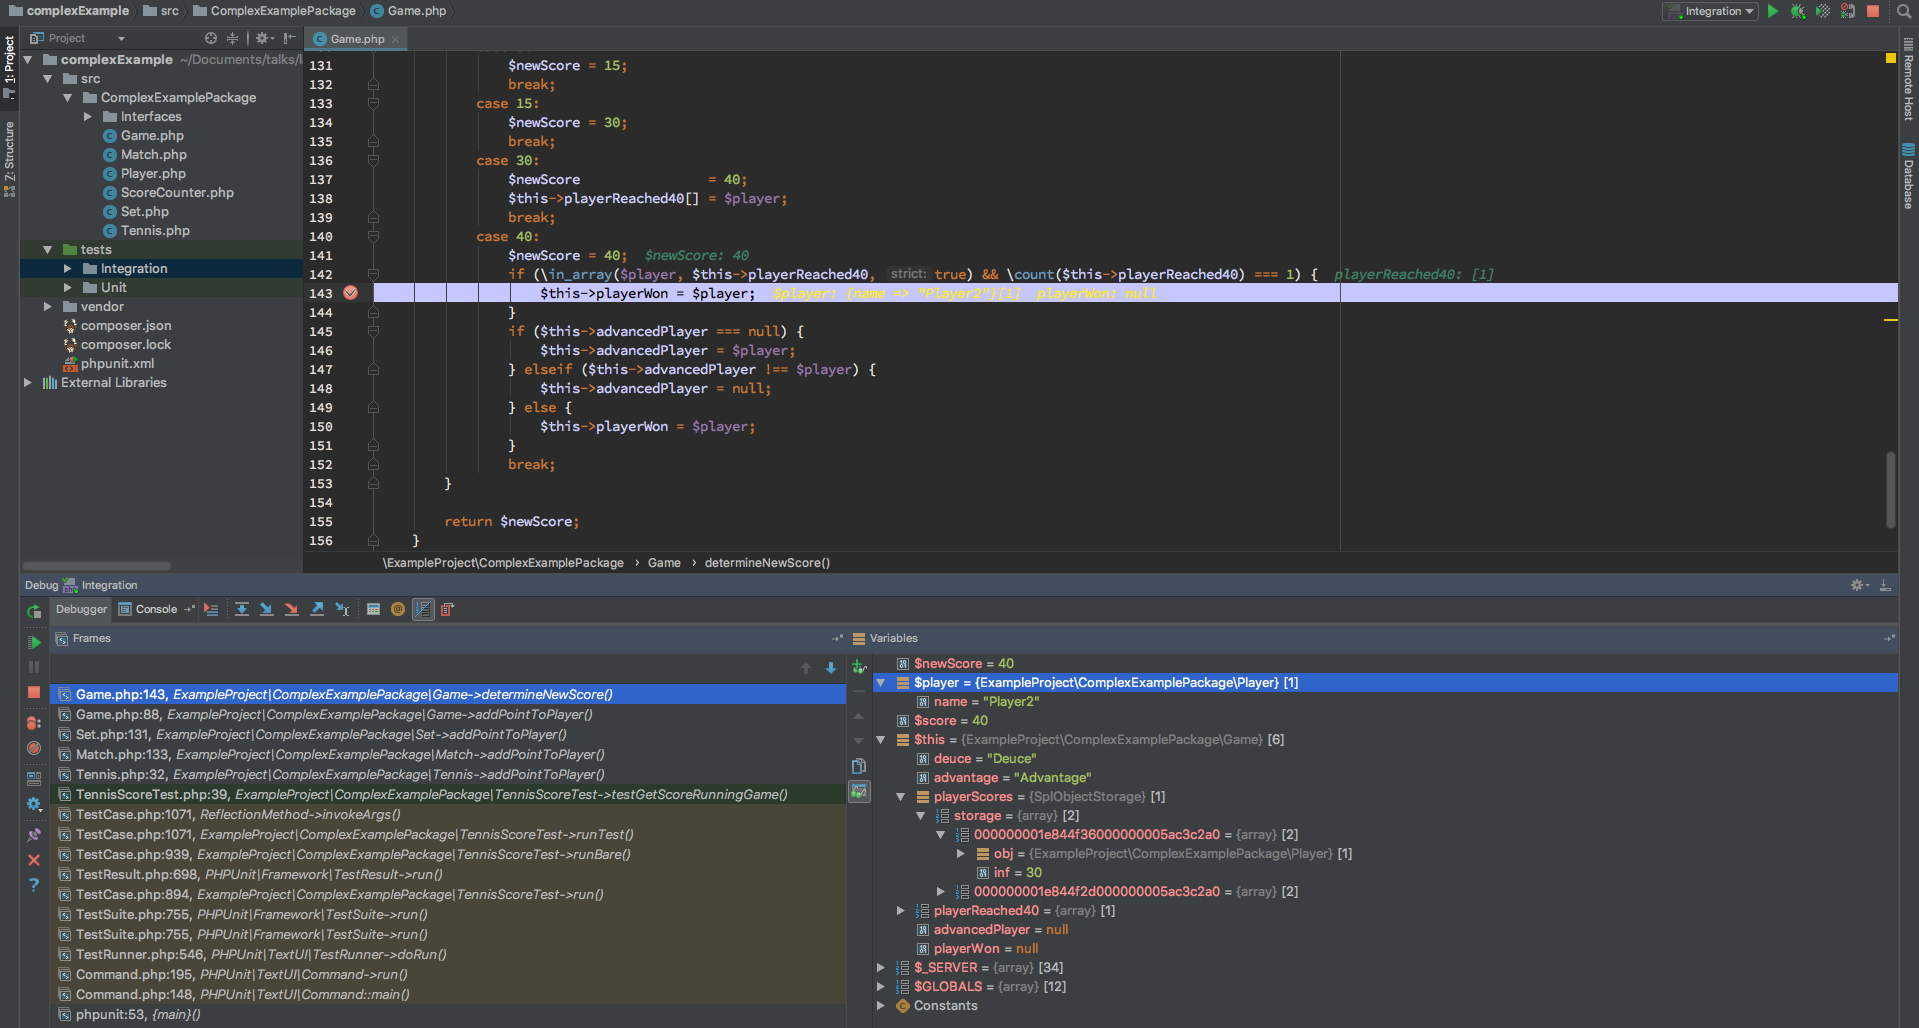
\includegraphics[height=12em]{phpstorm-debugging}
    \end{figure}
    \begin{multicols}{2}
    \begin{itemize}
      \item Steuern des Programmablaufs durch \dots
      \begin{itemize}
        \item Haltepunkte
        \item Schrittweises abarbeiten von Anweisungen
      \end{itemize}
      \columnbreak{}
      \item Inspizieren von Daten in flüchtigem Speicher
      \item Modifizieren von Daten und Programmcode
      \item \"{}Just in Time\"{}-Ausführung von Programmcode

    \end{itemize}
  \end{multicols}
\end{frame}


\subsection{Warum Xdebug}


\begin{frame}
  \frametitle{\secname}
  \framesubtitle{\subsecname}
    \begin{columns}
		\begin{column}{0.5\textwidth}
			\begin{figure}
				\begin{center}
					
\includegraphics[width=\textwidth]{meme-mean-kitten-debugger}
				\end{center}
			\end{figure}
		\end{column}
    	\begin{column}{0.5\textwidth}
    		\begin{itemize}
    		  \item Brauche ich nicht \\ \ldots macht das Leben aber einfacher
    		  \note[item]{Man braucht auch keine IDE und speichert Daten mit magnetisierter Nadel auf der Festplatte}
    		  \item \mintinline{php}|var_dump()| reicht mir \\ \ldots ist aber aufwendig, langsam und statisch
    		  \note[item]{debug code muss geschrieben und entfernt werden}
    		  \note[item]{debug code ist zur Laufzeit statisch}
    		  \note[item]{debug code steigt nicht beliebig tief in Objekte}
              \note[item]{Arbeitsschritte ohne debugger: \\ error reporting an, \\ print hinzufügen, \\ Seite laden, \\ Ausgabe finden, \\Code anpassen, \\Ausgabe anpassen, \\ alles zurück bauen,}
    		\end{itemize}
    	\end{column}
    \end{columns}

\end{frame}


\section{Installation}
\subsection{PEAR/PECL}


\begin{frame}
  \frametitle{\subsecname}
  \framesubtitle{Voraussetzungen}

  Voraussetzungen für die Installation über PEAR

  \begin{itemize}
    \item Xdebug > 0.9.0
    \item PEAR > 0.9.1
    \item *nix System. Auf Windows nicht ohne weiteres möglich
  \end{itemize}

\end{frame}


\begin{frame}
  \frametitle{\subsecname}
  \framesubtitle{Installation}

  \begin{enumerate}
    \item \mintinline{bash}|pear install pecl/xdebug|
    \item Folgende Zeile zu \mintinline{bash}|php.ini| hinzufügen \\ \mintinline{bash}|zend_extension="/path/to/extension/xdebug.so"|
  \end{enumerate}

\end{frame}


\subsection{Brew / APT}


\begin{frame}
  \frametitle{\secname}
  \framesubtitle{\subsecname}

  In vielen *nix-Betriebssystemen kann man Xdebug auch über den Paketmanager beziehen. Hier zwei Beispiele für PHP 7.0. \\

  \sout{Mit \mintinline{bash}|brew| unter \alert{MacOS}} \\
  Seit brew 1.5 nicht mehr gepflegt.
    \begin{itemize}
      \item \mintinline{bash}|brew install php70-xdebug|
    \end{itemize}
  Mit \mintinline{bash}|apt-get| unter \alert{Ubuntu}
  \begin{itemize}
    \item \mintinline{bash}|sudo apt-get install php-xdebug|
  \end{itemize}
  ~\\
  \mintinline{bash}|php -m| Zeigt einem die installierten Erweiterungen an. Nach der Installation also auch Xdebug.

\end{frame}


\subsection{Binary}

\begin{frame}
  \frametitle{\subsecname}
  \framesubtitle{\subsecname}

  \begin{multicols}{2}
    Xdebug bietet auf ihrer Webseite einen wizard, mit dessen Hilfe man Xdebug selbst compilieren kann.

    \begin{enumerate}
      \item \chref{https://xdebug.org/wizard.php}{Wizard öffnen}
      \item Ausgabe von \mintinline{bash}|php -i| in die Textbox kopieren
      \item Anweisungen auf dem Bildschirm folgen
    \end{enumerate}
    \begin{figure}
      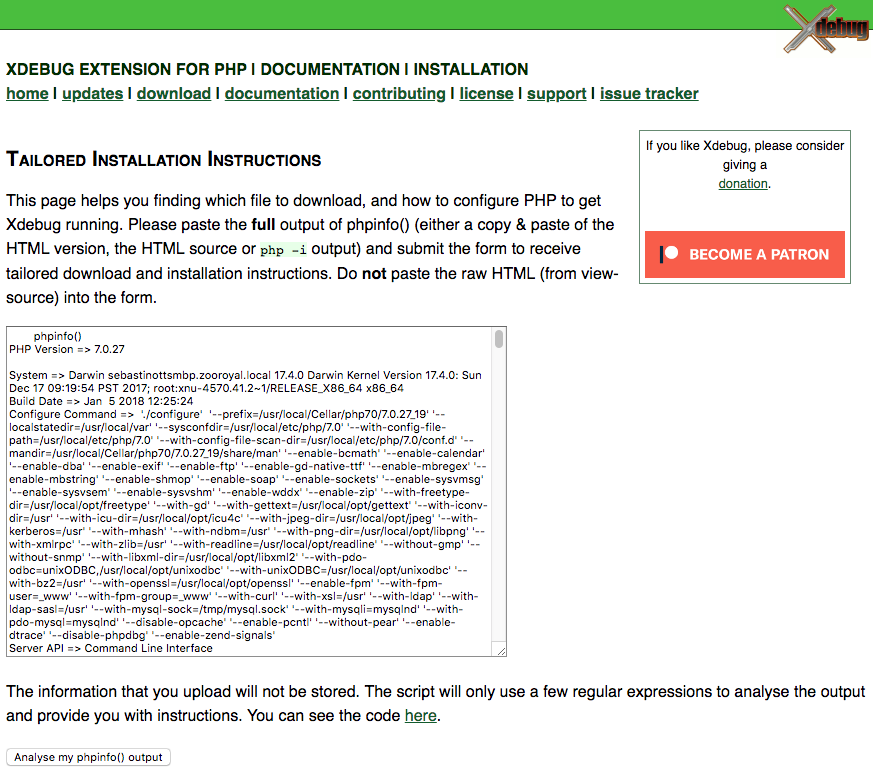
\includegraphics[width=14em]{xdebug-wizard}
    \end{figure}
  \end{multicols}
\end{frame}

\subsection{Konfiguration}


\begin{frame}
  \frametitle{\secname}
  \framesubtitle{\subsecname}

  \begin{figure}
    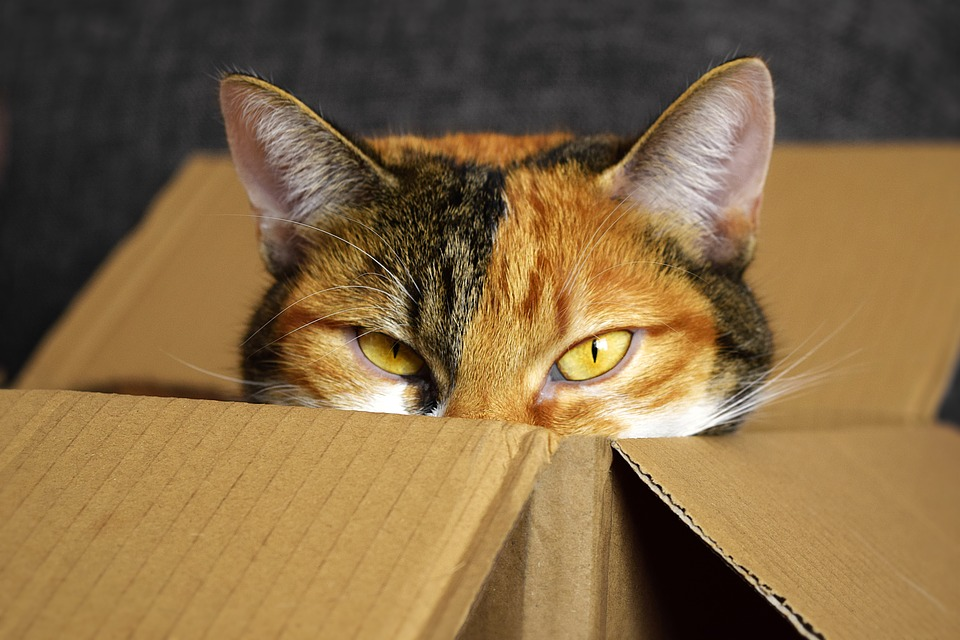
\includegraphics{out-of-the-box}
  \end{figure}

  Die Konfiguration für lokale PHP-Interpreter läuft \alert{out-of-the-box}.
\end{frame}


\begin{frame}
  \frametitle{\secname}
  \framesubtitle{Remote Debugging}

  \begin{figure}
    \includegraphics<1>[width=\textwidth]{dbgp-remote-debug-0}
    \note<1>[item]{Zwei Rechner; einer für die IDE, einer für den PHP-Interpreter}
    \note<1>[item]{Port 80 offen für den Webserver}
    \includegraphics<2>[width=\textwidth]{dbgp-remote-debug-1}
    \note<2>[item]{xdebug.connect\_back = 1 in die PHP.ini}
    \includegraphics<3>[width=\textwidth]{dbgp-remote-debug-2}
    \note<3>[item]{IDE Rechner muss Port 9000 offen haben}
    \note<3>[item]{xdebug.remote\_port = 9000}
    \includegraphics<4>[width=\textwidth]{dbgp-remote-debug-3}
    \note<4>[item]{Aufruf der Webseite}
    \includegraphics<5>[width=\textwidth]{dbgp-remote-debug-4}
    \note<5>[item]{Xdebug verbindet sich mit IDE}
    \includegraphics<6>[width=\textwidth]{dbgp-remote-debug-5}
    \note<6>[item]{Server antwortet schrittweise auf HTTP-Request}
  \end{figure}

  Der Webserver auf dem der PHP-Interpreter läuft ist nicht der selbe Rechner auf dem entwickelt wird.
  \begin{itemize}
    \item Lösung per Remote Debugging
    \item Konfiguration in php.ini
  \end{itemize}
\end{frame}


\begin{frame}
  \frametitle{\secname}
  \framesubtitle{\subsecname}
  \begin{multicols}{2}
    \begin{figure}
      \includegraphics<1>[width=15em]{meme-thinking}
      \includegraphics<2>[width=15em]{meme-thumbs-up}
    \end{figure}
    \columnbreak{}
    Was müsst ihr jetzt tun wenn ihr in der ZooRoyal-Devbox debuggen wollt?

    \begin{itemize}
      \item<2> Einfach Alexander Fitzkes \chref{https://confluence.rdss.it/display/DEV/Debugging}{Anleitung im Wiki} folgen.
    \end{itemize}
  \end{multicols}

\end{frame}


\section{Funktionen}
\subsection{Interactive Debugging}
\subsubsection{Breakpoints}


\begin{frame}[<+->]
  \frametitle{\subsecname}
  \framesubtitle{\subsubsecname}

  Breakpoint halten die Application an einer \alert{beliebigen Operation} an
  \begin{itemize}
    \item Analyse des Speichers
    \item Analyse des Call Stacks
    \item Ausführen von PHP-Code
    \item Schrittweises ausführen
  \end{itemize}
\end{frame}


\begin{frame}
  \frametitle{\subsubsecname}
  \framesubtitle{Step Into}
  \begin{columns}
    \begin{column}{0.4\textwidth}
      \begin{figure}
        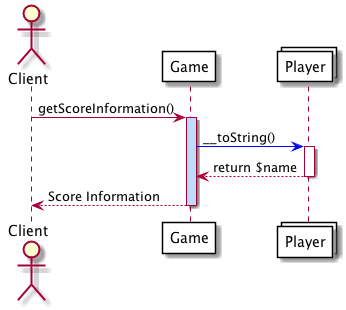
\includegraphics[width=\textwidth]{step-into}
      \end{figure}
    \end{column}
    \begin{column}{0.6\textwidth}
      \begin{itemize}[<+->]
        \item Die Applikation hält in einem Breakpoint in Game \inputminted[firstline=64,lastline=64,linenos=false]{php}{complexExample/src/ComplexExamplePackage/Game.php}
        \item Mit \alert{step into} steigt der Debugger den Callstack eine Ebene herab
        \item Applikation hält in der ersten Zeile von \mintinline{php}|player->__toString|
      \end{itemize}
    \end{column}
  \end{columns}
\end{frame}


\begin{frame}
  \frametitle{\subsubsecname}
  \framesubtitle{Step Over}
  \begin{columns}
    \begin{column}{0.4\textwidth}
      \begin{figure}
        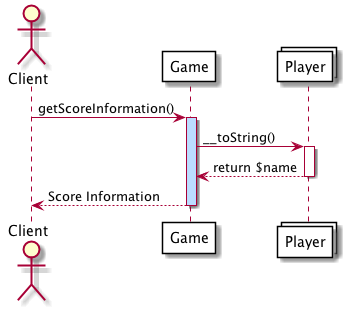
\includegraphics[width=\textwidth]{step-over}
      \end{figure}
    \end{column}
    \begin{column}{0.6\textwidth}
      \begin{itemize}[<+->]
        \item Die Applikation hält in einem Breakpoint in Game
        \item Mit \alert{step over} bleibt der Debugger auf der \alert{selben Ebene des Callstack}
        \item Applikation führt Operation am Breakpoint aus und hält in der nächsten Zeile in Game
      \end{itemize}
    \end{column}
  \end{columns}
\end{frame}


\begin{frame}
  \frametitle{\subsubsecname}
  \framesubtitle{Step Out}
  \begin{columns}
    \begin{column}{0.4\textwidth}
      \begin{figure}
        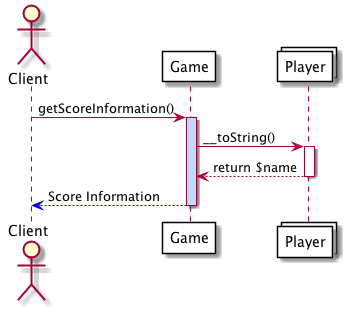
\includegraphics[width=\textwidth]{step-out}
      \end{figure}
    \end{column}
    \begin{column}{0.6\textwidth}
      \begin{itemize}[<+->]
        \item Die Applikation hält in einem Breakpoint in Game
        \item Mit \alert{step out} steigt der Debugger \alert{eine Ebene im Callstack auf}
        \item Applikation führt alle Operationen auf der aktuellen Ebene des Callstacks aus und hält an der nächsten Operation der nächst höheren Ebene.
      \end{itemize}
    \end{column}
  \end{columns}
\end{frame}


\begin{frame}
  \frametitle{\subsecname}
  \framesubtitle{\subsubsecname}
  \begin{figure}
    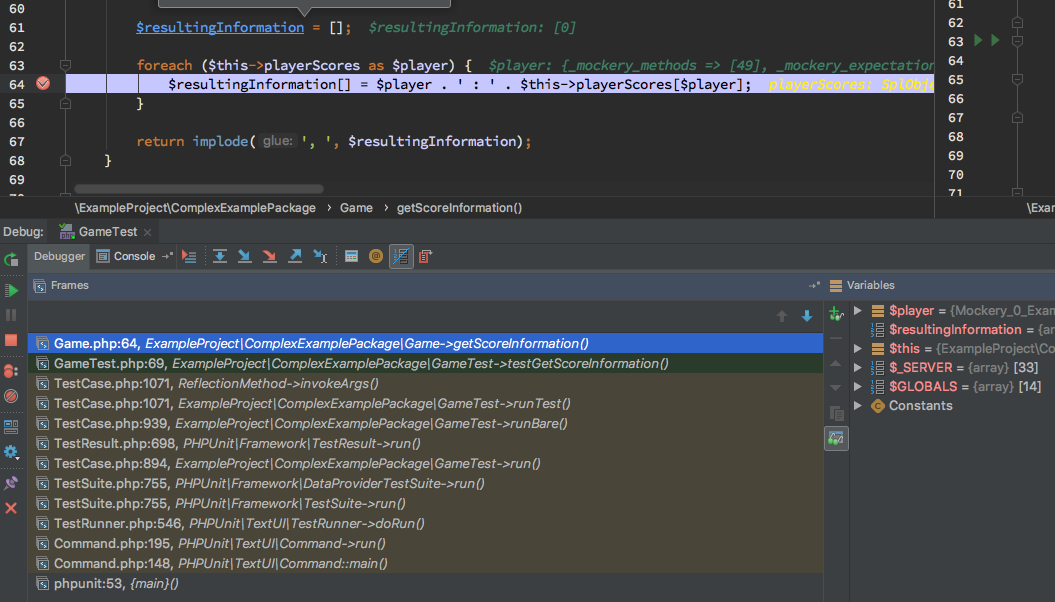
\includegraphics[width=\textwidth]{phpstorm-breakpoint}
  \end{figure}
  \note{Wechsel zu PHPStorm complexExample/*/Game.php und Test Zeile 88}
\end{frame}


\begin{frame}
  \frametitle{\secname}
  \framesubtitle{\subsecname}

  \begin{figure}
    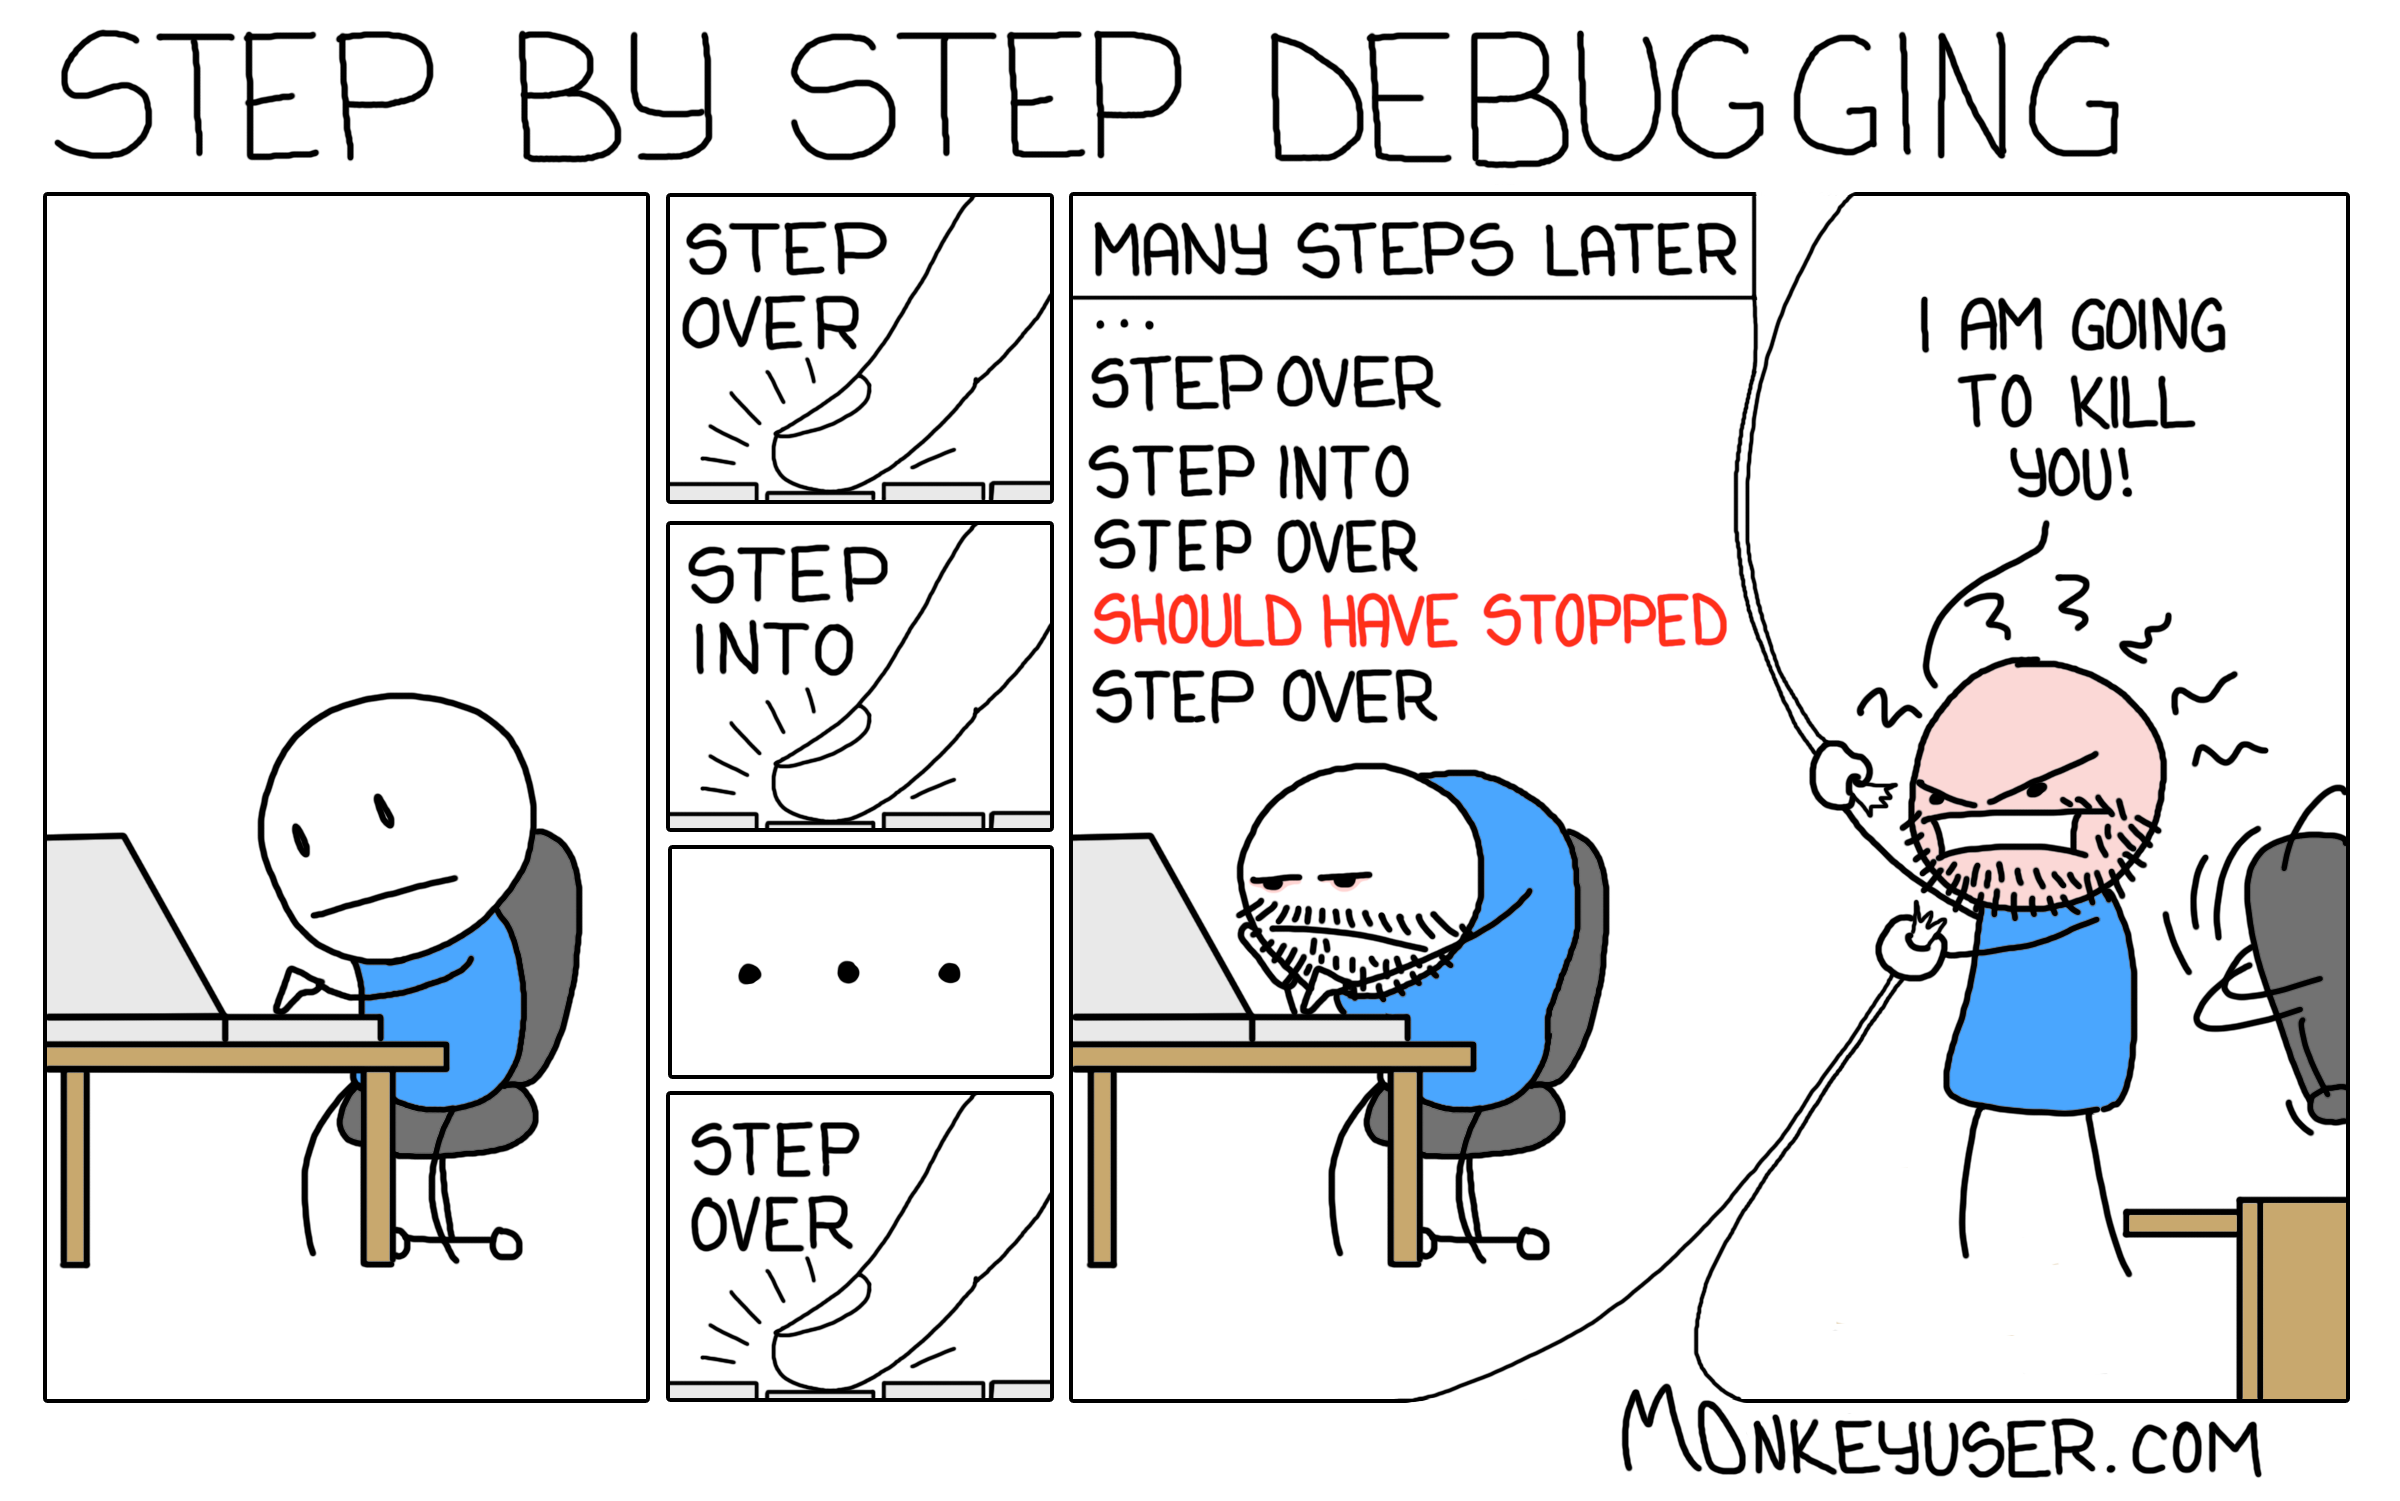
\includegraphics[width=\textwidth]{comic-debug}
  \end{figure}
\end{frame}


\subsubsection{Conditions}


\begin{frame}
  \frametitle{\subsecname}
  \framesubtitle{\subsubsecname}
  In bestimmt Situation möchte man die Application an einer Stelle nur unter \alert{bestimmten Umständen} anhalten
  \begin{itemize}[<+->]
    \item Rekursionen
    \note[item]{\chref{https://sourcemaking.com/design_patterns/composite}{Composite Pattern}}
    \item Schleifen
    \note[item]{Lange for- oder while-Schleifen}
    \item Exceptions
    \note[item]{Nur im Fehlerfall}
    \item In vielen Kontexten genutzter Code
    \note[item]{symfony/finder wird in vielen verschiedenen Kontexten benutzt}
  \end{itemize}
\end{frame}


\begin{frame}
  \frametitle{\subsecname}
  \framesubtitle{\subsubsecname}
  \begin{figure}
    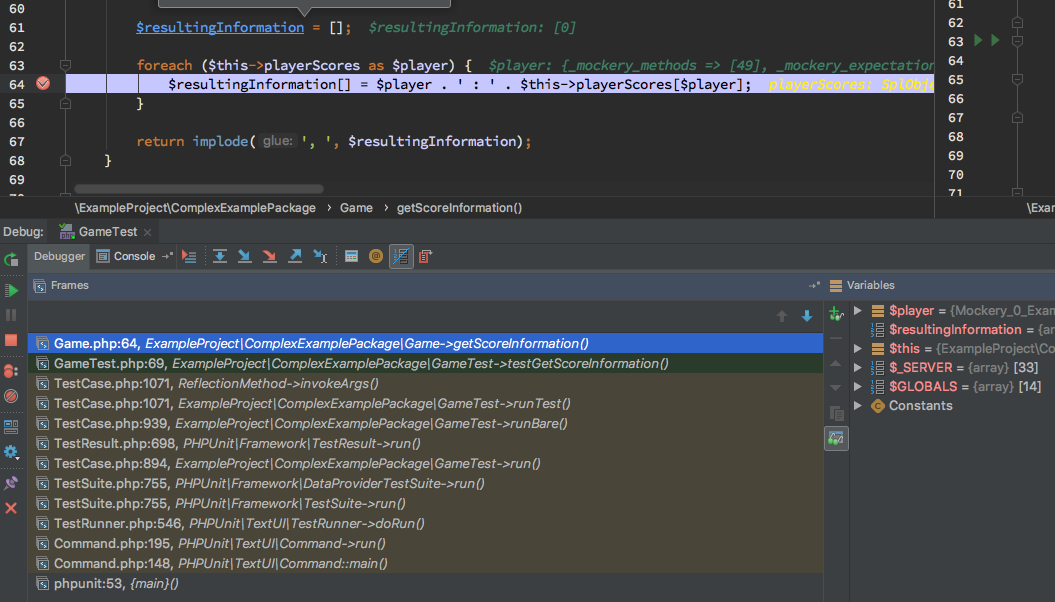
\includegraphics[width=\textwidth]{phpstorm-breakpoint}
  \end{figure}
  \note[item]{Wechsel zu PHPStorm complexExample/*/GameTest.php Zeile 71 \\
    Condition: \mintinline{php}|scoreCount === 3|
  }
  \note[item]{Wechsel zu PHPStorm complexExample/*/Game.php Zeile 49 \\
    Condition: Vorheriger Breakpoint
  }
\end{frame}


\subsubsection{Watches}


\begin{frame}
  \frametitle{\subsecname}
  \framesubtitle{\subsubsecname}
  \begin{figure}
    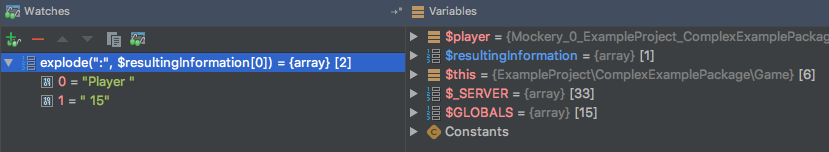
\includegraphics[width=\textwidth]{phpstorm-watches}
  \end{figure}
  \begin{itemize}[<+->]
    \item Watches sind kleine PHP Snippets
    \item Werden an jedem Haltepunkt ausgeführt
    \item Ausgabe wird dem Entwickler dargestellt
  \end{itemize}
\end{frame}

\begin{frame}
  \frametitle{\subsecname}
  \framesubtitle{\subsubsecname}
  \begin{figure}
    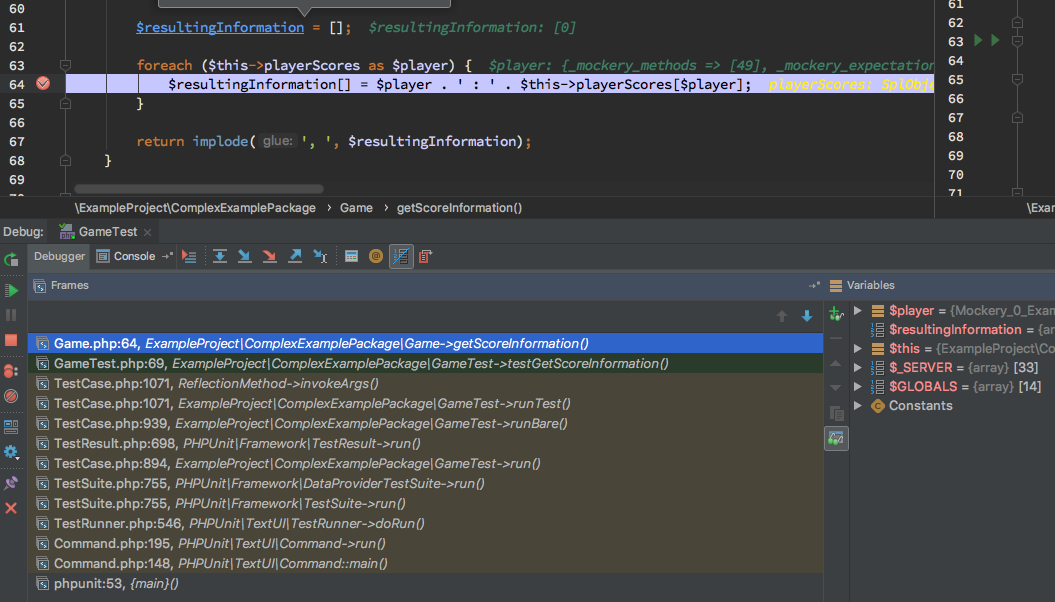
\includegraphics[width=\textwidth]{phpstorm-breakpoint}
  \end{figure}
  \note[item]{Wechsel zu PHPStorm complexExample/*/Game.php}
  \note[item]{64 Breakpoint}
  \note[item]{watch \mintinline{php}{\$resultingInformation}}
  \note[item]{watch \mintinline{php}|\$resultingInformation[0]|}
  \note[item]{watch \mintinline{php}|explode(":", \$resultingInformation[0])|}
\end{frame}


\subsubsection{Code Execution}


\begin{frame}
  \frametitle{\subsecname}
  \framesubtitle{\subsubsecname}

  \begin{figure}
    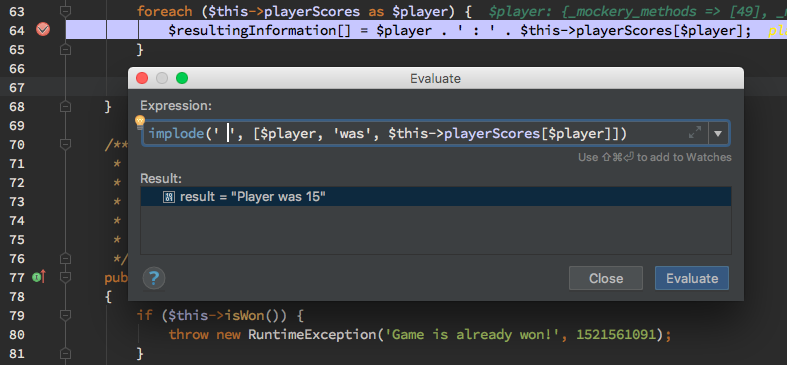
\includegraphics[height=12em]{phpstorm-execute-code}
  \end{figure}

  Ausführen von PHP-Code, wenn die Applikation angehalten wurde.
  \begin{itemize}[<+->]
    \item Zugriff auf Objekte im Scope
    \item Einfluss auf Programmablauf
    \item Direkte Ausgabe
  \end{itemize}
\end{frame}


\begin{frame}
  \frametitle{\subsecname}
  \framesubtitle{\subsubsecname}
  \begin{figure}
    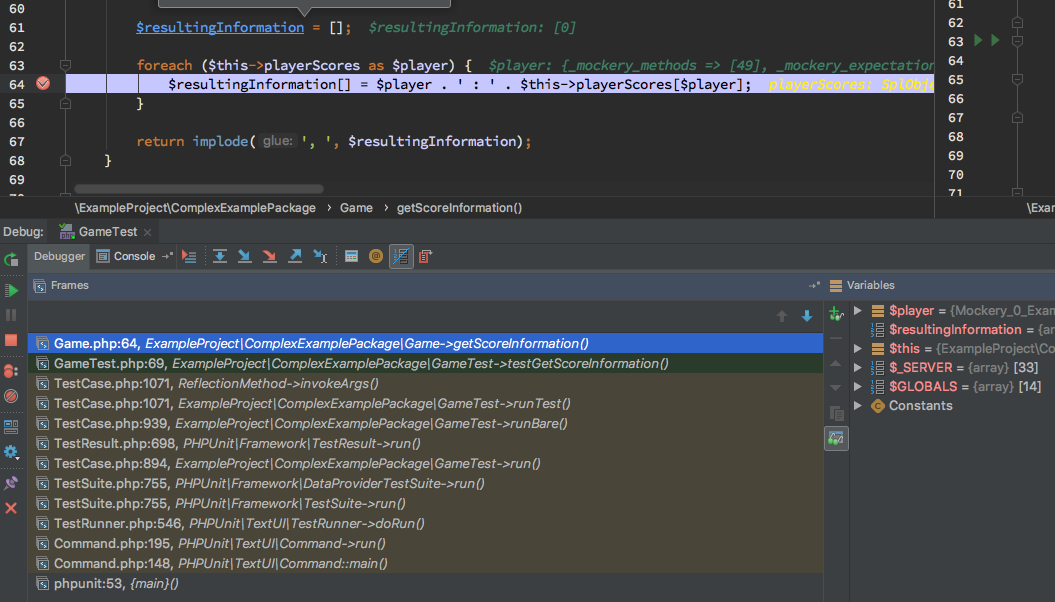
\includegraphics[width=\textwidth]{phpstorm-breakpoint}
  \end{figure}
  \note[item]{Wechsel zu PHPStorm complexExample/*/GameTest.php Zeile 64 \\
    \begin{itemize}
      \item Execution: \mintinline{php}|implode(1 + 5)|
      \item Execution: \mintinline{php}|implode(' ', [$player, 'was', $this->playerScores[$player]])|
      \item Execution: \mintinline{php}|implode(' ', [$player, 'was', $this->playerScores[$player]])|
    \end{itemize}
  }
\end{frame}


\subsection{Stack Trace}


\begin{frame}
  \frametitle{\secname}
  \framesubtitle{\subsecname}

  \begin{multicols}{2}
    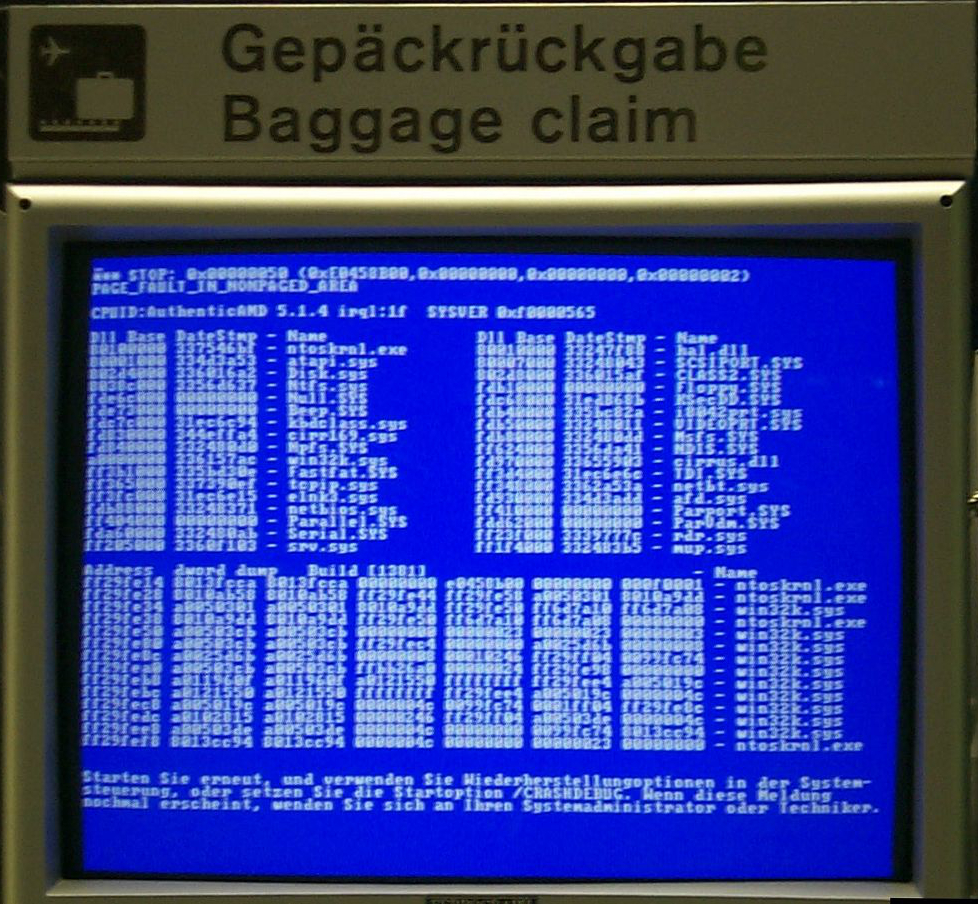
\includegraphics[width=0.5\textwidth]{stack-trace-gepaeck} \\
    \columnbreak{}

    Xdebug ergänzt die Ausgabe von Stack Traces um \dots
    \begin{itemize}
      \item Methodenparameter
      \item Lokale Variablen
      \item Superglobals
    \end{itemize}
  \end{multicols}
\end{frame}


\begin{frame}[plain]
  \vfill
  \inputminted{php}{Quellen/stack-trace.php}
  \vfill
\end{frame}


\begin{frame}[plain]
  \inputminted{php}{Quellen/stack-trace-php-output.txt}
\end{frame}


\subsection{Code Profiling}


\begin{frame}
  \frametitle{\secname}
  \framesubtitle{\subsecname}

  Xdebug kann für Aufrufe von PHP-Applikationen Ablaufprofile erzeugen.

  \begin{itemize}
    \item Call Tree
    \item Memory Allocation
    \item Time Tracking
  \end{itemize}

\end{frame}


\begin{frame}
  \frametitle{\subsecname}
  \framesubtitle{Konfiguration}

  Der Profiler muss mittels php.ini konfiguriert werden \\~\\
  \pause
  \mintinline{bash}{xdebug.profiler_enable=1}
  \begin{itemize}
    \item aktiviert den Profiler
  \end{itemize}
  \pause
  \mintinline{bash}{xdebug.profiler_enable_trigger=1}
  \begin{itemize}
    \item aktiviert den Profiler, wenn die richtig POST-, GET-, oder COOKIE-Variable gesetzt
  \end{itemize}
  \pause
  \mintinline{bash}{xdebug.profiler_output_dir=/path/asd}
  \begin{itemize}
    \item gibt den Speicherort für Profildateien an
  \end{itemize}
\end{frame}


\begin{frame}
  \frametitle{\subsecname}
  \framesubtitle{Call Tree}

  Mittels eines Call Trees kann der Entwickler nachvollziehen, welche Methoden in welcher Reihenfolge abgearbeitet worden sind.

\end{frame}


\subsection{Code Coverage Analysis}


\begin{frame}
  \frametitle{\secname}
  \framesubtitle{\subsecname}
\end{frame}


%-------------------------------------------------------
% HELPER PAGES
%-------------------------------------------------------

\appendix

\begin{frame}<handout:0>[label=5minPause]
  \frametitle{Pause}
  \framesubtitle{5 Minuten Pause}
  \begin{figure}
    \begin{center}
      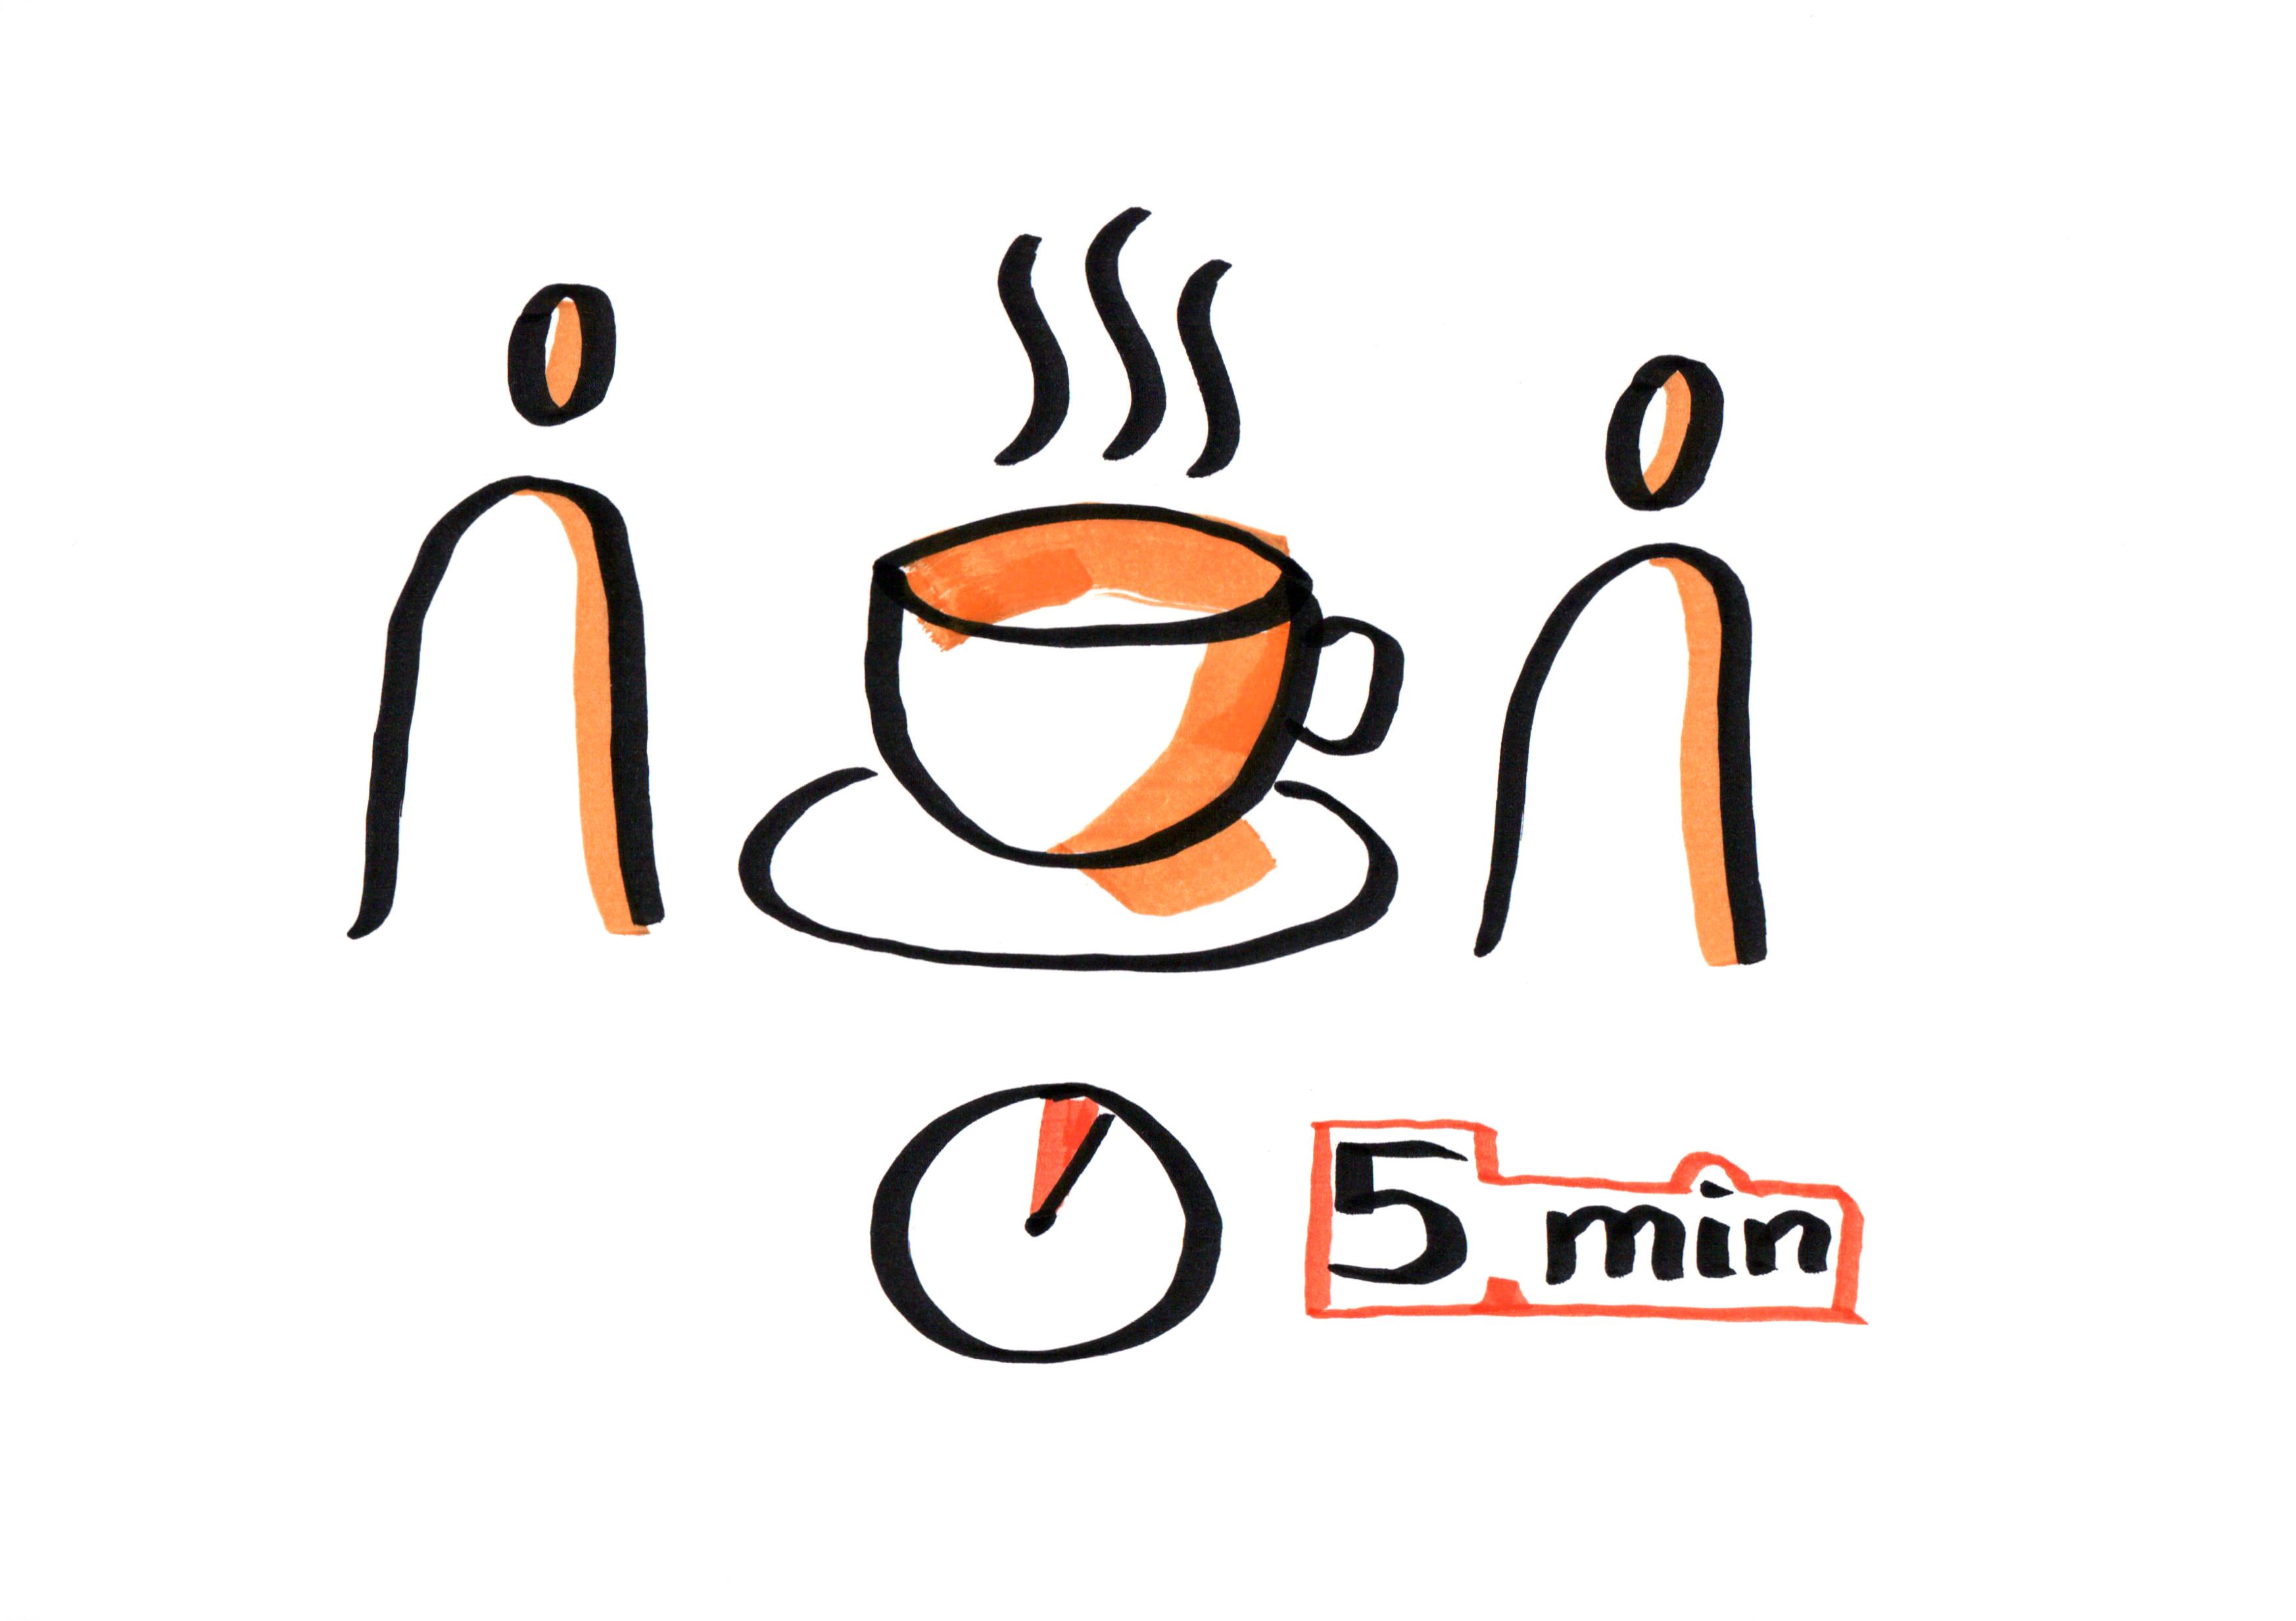
\includegraphics[height=4cm]{pause-5-min}
    \end{center}
  \end{figure}
\end{frame}



\begin{frame}<handout:0>[label=10minPause]
  \frametitle{Pause}
  \framesubtitle{10 Minuten Pause}
  \begin{figure}
    \begin{center}
      
\includegraphics[height=4cm]{pause-10-min}
    \end{center}
  \end{figure}
\end{frame}



\begin{frame}<handout:0>[label=pause]
  \frametitle{Pause}
  \framesubtitle{Pause}
  \begin{figure}
    \begin{center}
      
\includegraphics[height=4cm]{pause}
    \end{center}
  \end{figure}
\end{frame}



\begin{frame}<handout:0>[label=fragen,fragile]
  \frametitle{Fragen}
  \framesubtitle{Fragen?}
  \begin{figure}
    \begin{center}
      
\includegraphics[height=4cm]{fragen}
    \end{center}
  \end{figure}
\end{frame}



\end{document}

\end{document}
